%!TEX root = ../main.tex

\chapter{Kravspecifikation}

\RevisionsTabel{Kravspecifikation}{
Alle	& 1	 	& 23-02-2015  \\
Alle	& 2		& 19-04-2015  \\
		& 		&   \\
		& 	 	&   \\
}

%Aktører
\section{Aktører}
%!TEX root = ../../main.tex

I dette afsnit beskrives aktører og deres rolle i systemet. I figur \ref{photo:Aktor} ses aktørdiagram, som beskriver alle aktører og deres forhold til systemet


\begin{figure}[H]
	\centering
	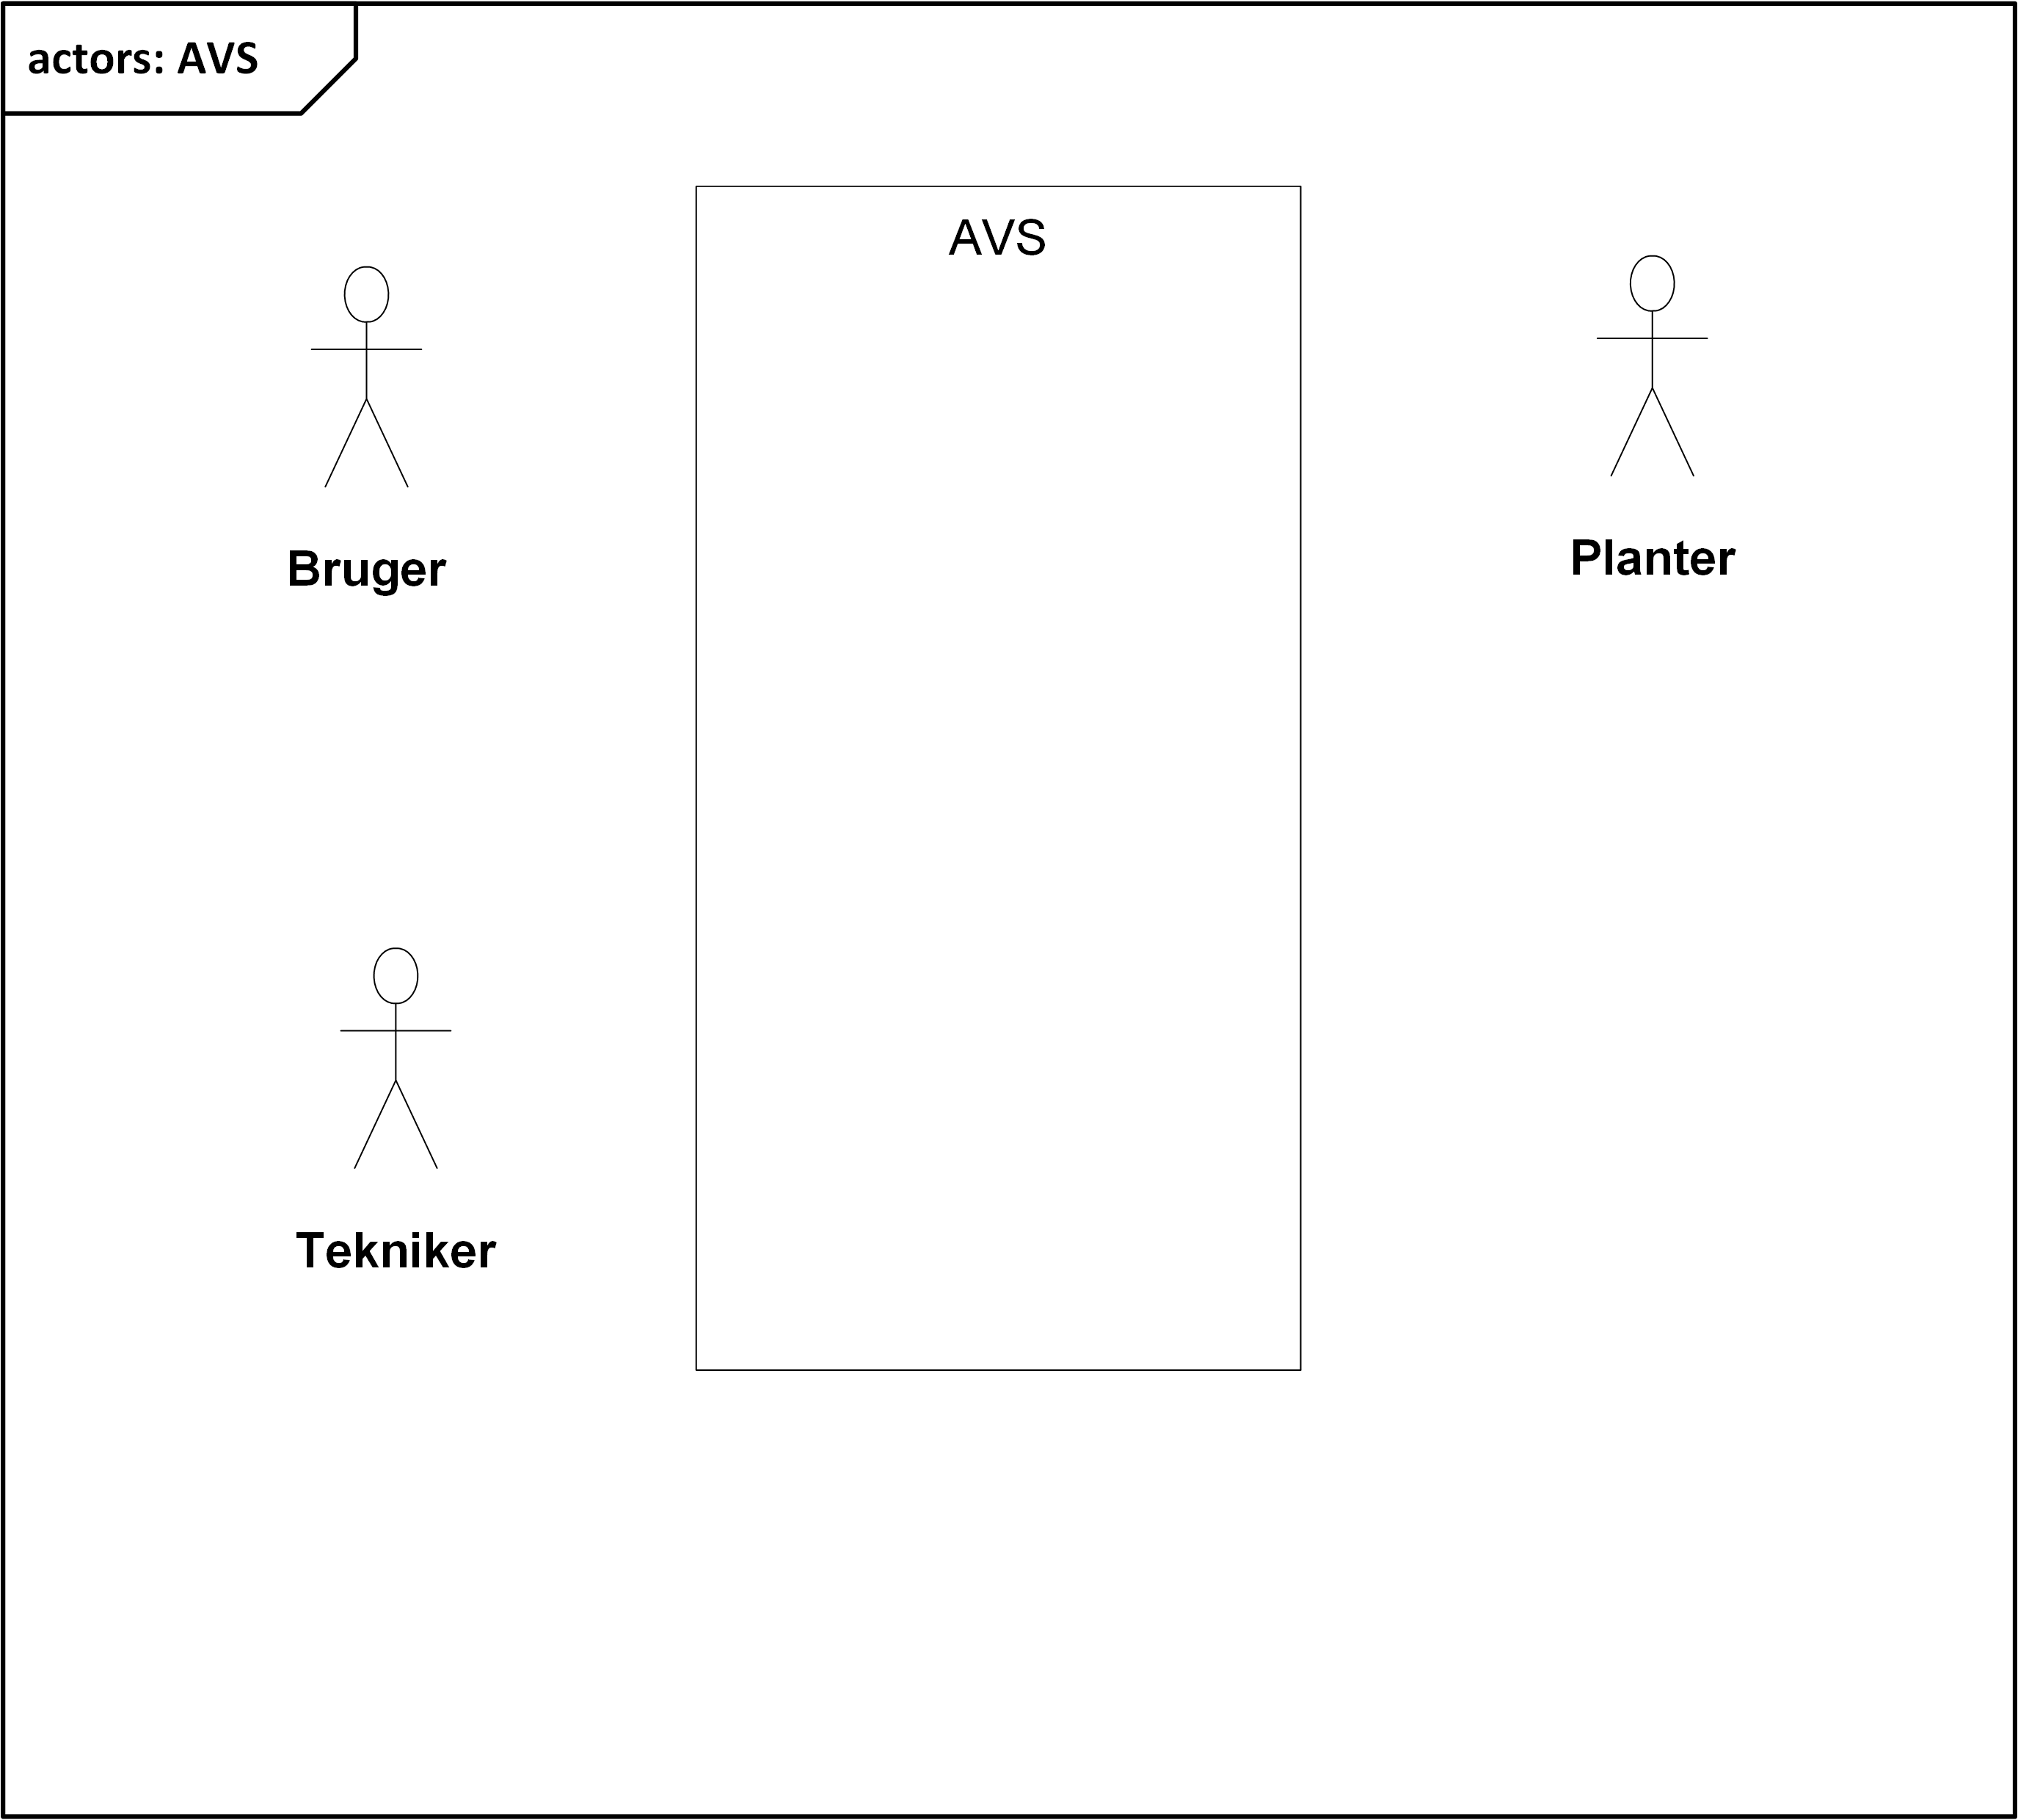
\includegraphics[scale=1]{Kravspecifikation/Actor/Photo/AVS_Actors}
	\caption{AVS Aktører}
	\label{photo:Aktor}
\end{figure}

\newpage

\subsection{Bruger}
\begin{usecase}
\addtitle{Aktørnavn}{Bruger} 
\addfield{type:}{Primær}
\addfield{Beskrivelse:}{Bruger er ham, som til dagligt tilgår systemet. Han ved hvor meget gødning og fugtighed planterne skal have, og angiver disse værdier i brugergrænsefladen. Det er brugeren som løbende ændrer værdierne, så systemet hele tiden er opdateret med værdier der passer til planternes vækststadier.}
\end{usecase}

\subsection{Tekniker}
\begin{usecase}
\addtitle{Aktørnavn}{Tekniker} 
\addfield{type:}{Primær}
\addfield{Beskrivelse:}{Tekniker er en specielt uddannet person. Han har den nødvendige viden om systemet til at kunne installere systemet fra opstart, opsætte nye vandkar mv. En Bruger kan også være tekniker.}
\end{usecase}






%Use Cases
\newpage
\section{Use Cases}
%	Indledning
I dette afsnit ses de forskellige Use Cases. På billede \ref{photo:UseCD} ses et Use case diagram, som viser en simpel repræsentation af bruger, tekniker og \glslink{plante}{planters} interaktion med systemet og en afbildning af de forskellig Use Cases. 



\begin{figure}[H]
	\centering
	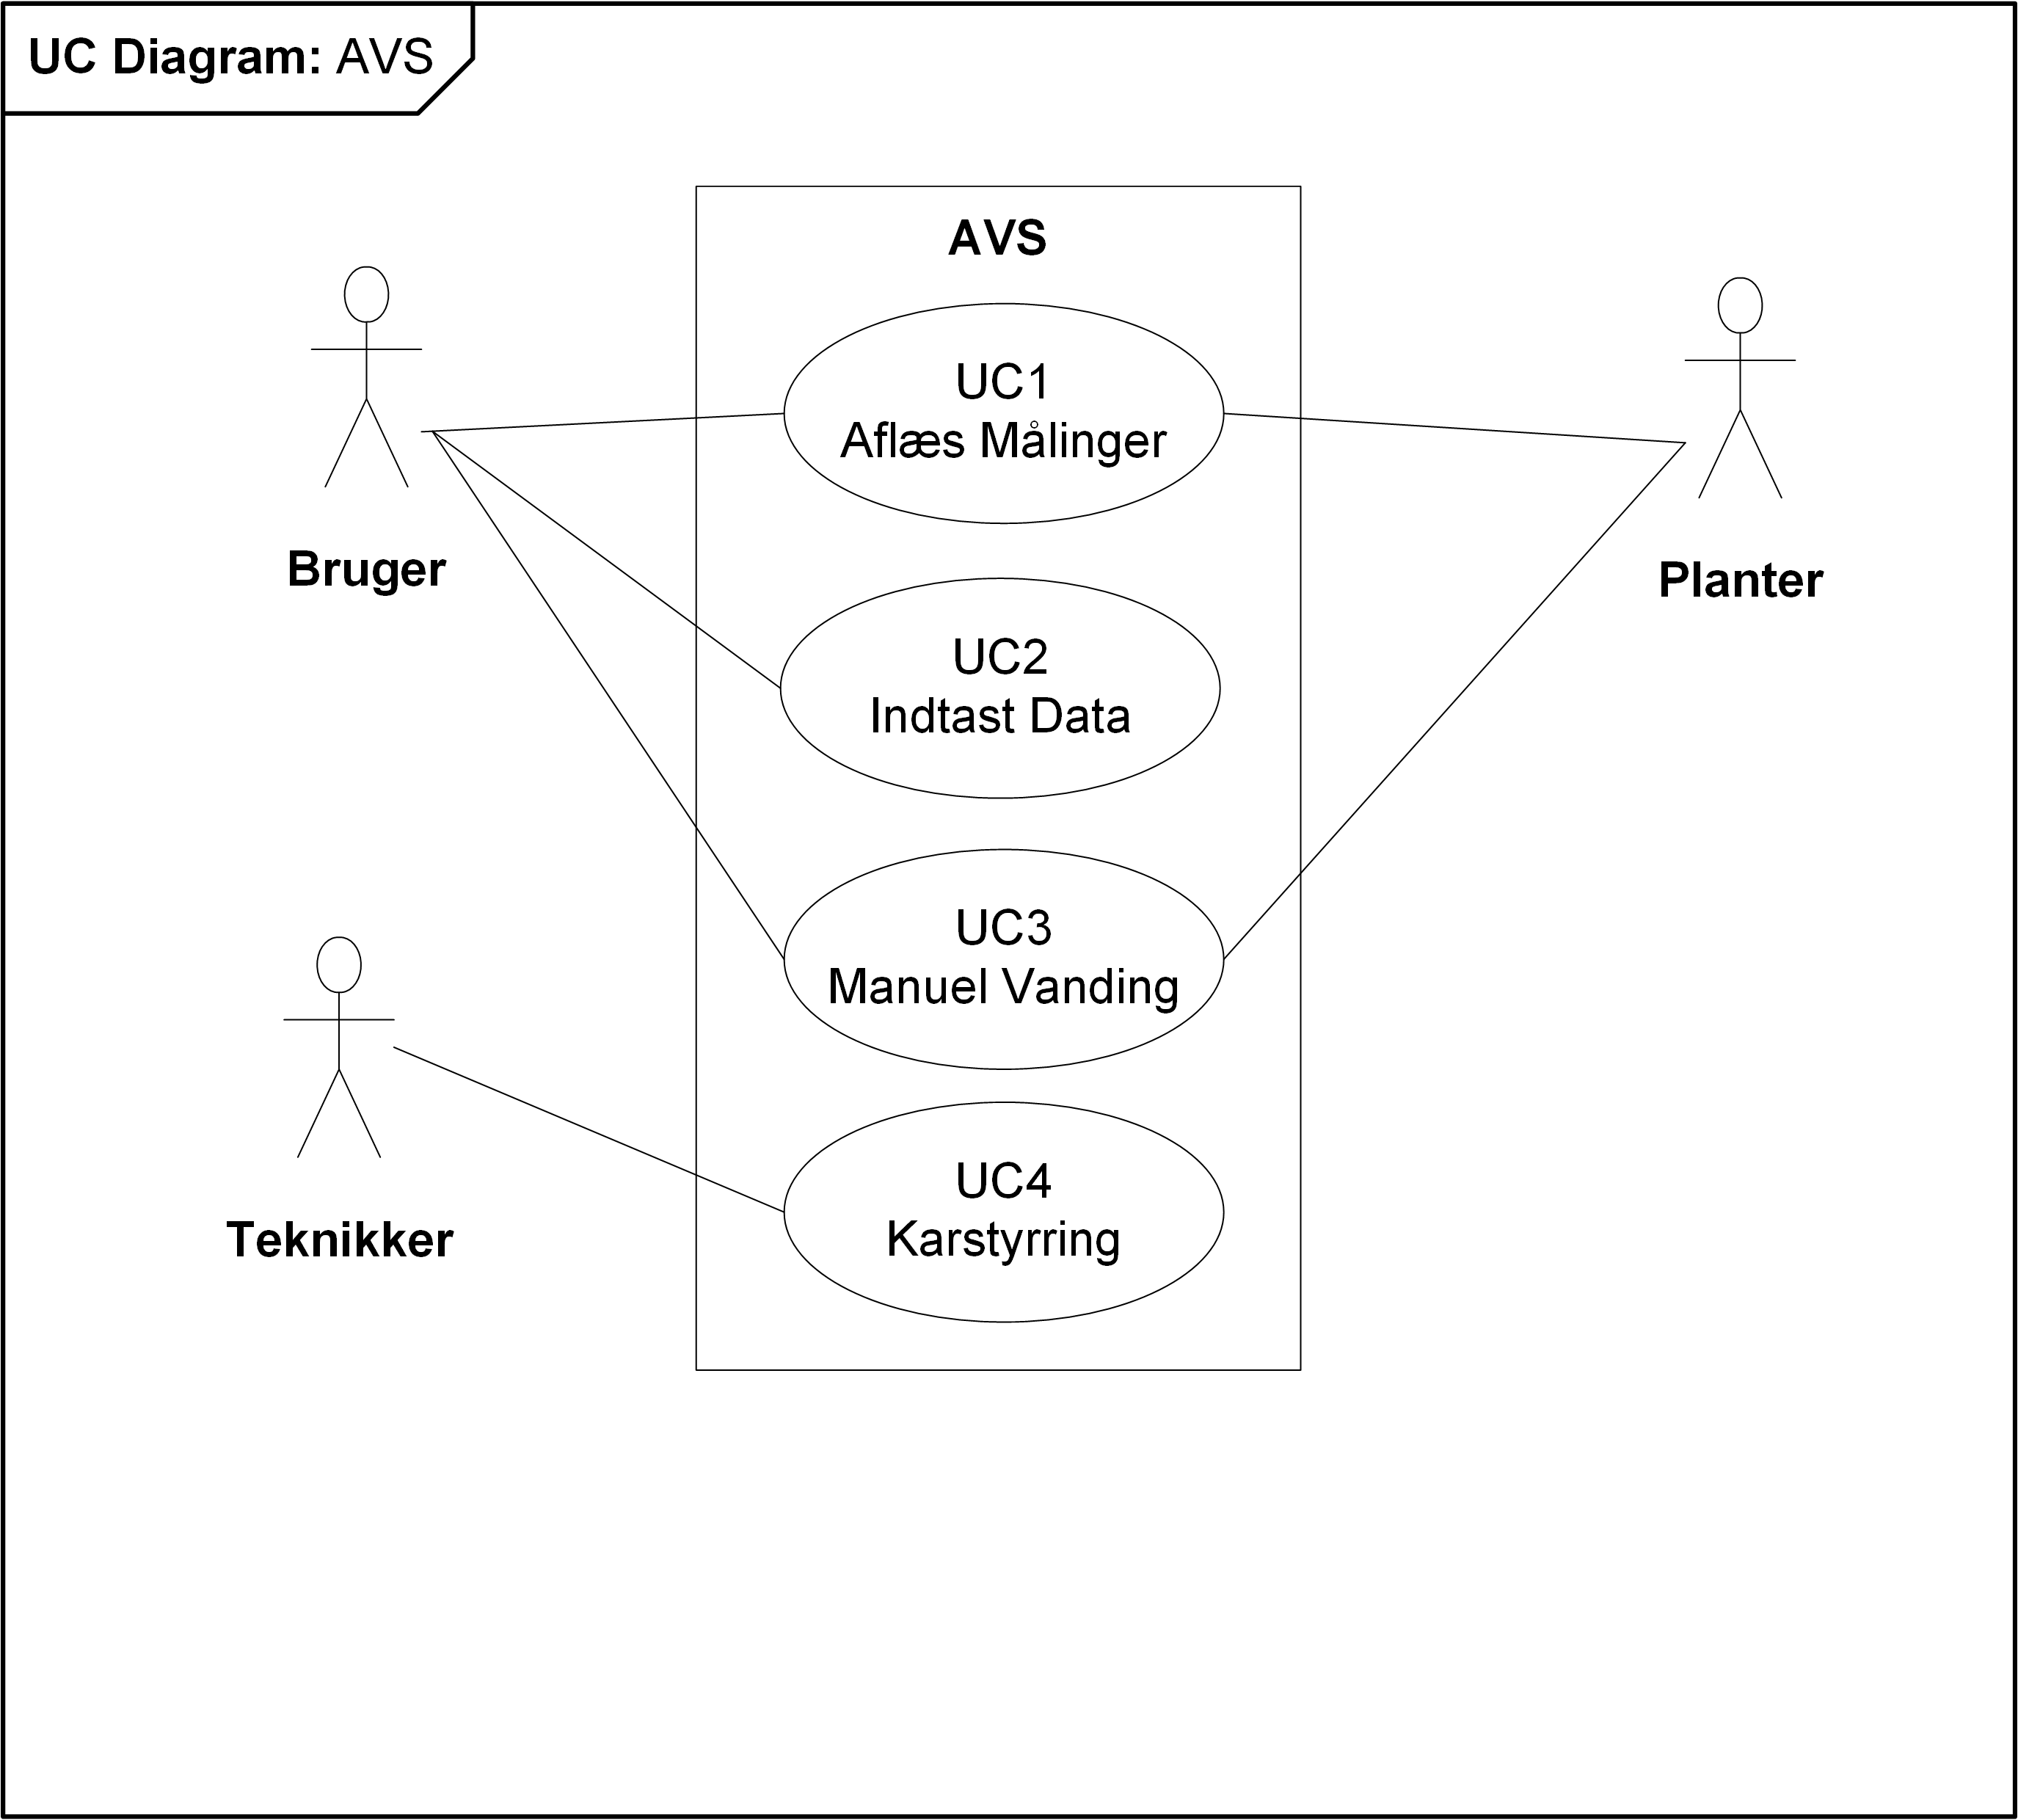
\includegraphics[scale=1]{Kravspecifikation/UseCases/Photo/AVS_UseCases}
	\caption{AVS Use case diagram}
	\label{photo:UseCD}
\end{figure}

\newpage
%	#1 Aflæs målinger
\subsection{Usecase 1}
Beskrivelse af denne use case
\begin{usecase}

\addtitle{Use Case 1}{Aflæs målinger} 

\addfield{Goal:}{mål!}

\additemizedfield{Initiatet by:}{
	\item bruger
	\item noget
}

\addfield{Actors:}{End-User}

\addfield{Concurrent occurances:}{1}

%Preconditions: What must be true on start and worth telling the reader?
\addfield{Preconditions:}{}

%Postconditions: What must be true on successful completion and worth telling the reader
\addfield{Postconditions:}{}

%Main Success Scenario: A typical, unconditional happy path scenario of success.
\addscenario{Main Success Scenario:}{
	\item The first action
	\item The second action
}

%Extensions: Alternate scenarios of success or failure.
\addscenario{Extensions:}{
	\item[2.a] Invalid login data:
		\begin{enumerate}
		\item[1.] System shows failure message
		\item[2.] User returns to step 1
		\end{enumerate}
	\item[5.a] Invalid subsriber data:
		\begin{enumerate}
		\item[1.] System shows failure message
		\item[2.] User returns to step 2 and corrects the errors
		\end{enumerate}
}


\end{usecase}

%	#2 Manuel vanding
\newpage
\subsection{Use case 2}
I denne use case ønsker brugeren at tilføre vand manuelt til planterne. Denne use case kan kun tilgås af en person. For at denne use case kan gennemføres skal der være vand i det kar der ønskes at vande fra samt at dette er tilføjet til systemet. Karet skal være koblet på mindst en sensor ø.
\begin{usecase}

\addtitle{Use Case 2}{Manuel vanding} 

\addfield{Mål:}{At tilføre vand til planterne}

\additemizedfield{Initieret af:}{
	\item Bruger
}

\addfield{Aktør:}{Bruger}

\addfield{Samtidige forekomster:}{1}

%Preconditions: What must be true on start and worth telling the reader?
\addfield{Prækondition:}{Der skal være vand i det kar der ønskes at vande fra og der skal være tilkoblet mindst en sonsor ø. GUI'en befinder sig i hovedmenuen}

%Postconditions: What must be true on successful completion and worth telling the reader
\addfield{Postkonditions:}{Der er vand ved planterne}

%Main Success Scenario: A typical, unconditional happy path scenario of success.
\addscenario{Hovedscenario:}{
	\item Bruger trykker på "Kar X" i GUI
	\item Systemet viser et skærmbillede hvor der kan vælges manuel vanding
	\item Bruger trykker på "Manuel vanding"
	\item Systemet begynder at vande
	\item Systemet ændre knappen for manuel vanding til stop maunel vanding
	\item[ ] [Ex.1 Karret er tomt]
	\item Når der ikke ønskes at vande længere trykker bruger på "Stop manuel vanding"
	\item Systemet stopper med at vande
}

%Extensions: Alternate scenarios of success or failure.
\addscenario{Udvidelser:}{
	\item[Ex.1] Karret er tomt:
		\begin{enumerate}
		\item[1.] Systemet stopper med at vande
		\end{enumerate}
}


\end{usecase}

%	#3 Indtast pH
\newpage
\subsection{Use case 3}
I denne use case ønsker brugeren at tilføre vand manuelt til planterne. Denne use case kan kun tilgås en person, der der kun er en interface. For at denne use case kan gennemløbes skal der være vand i det kar der ønskes at vandes fra og der er indtastet systemdata som blev indtastet i use case 2.
\begin{usecase}

\addtitle{Use Case 3}{Manuel vanding} 

\addfield{Mål:}{At tilføre planterne vand}

\additemizedfield{Initieret af:}{
	\item Bruger
}

\addfield{Aktør:}{Bruger}

\addfield{Samtidige forekomster:}{1-Antal \gls{vandkar}}

%Preconditions: What must be true on start and worth telling the reader?
\addfield{Prækondition:}{Der skal være vand i det kar der ønskes at vande fra. Der er indtastet system data fra UC2.}

%Postconditions: What must be true on successful completion and worth telling the reader
\addfield{Postkonditions:}{Der er vand ved planterne}

%Main Success Scenario: A typical, unconditional happy path scenario of success.
\addscenario{Hovedscenario:}{
	\item Bruger tilgår systemet via \glslink{gui}{gui'en}
	\item Bruger vælger i menuen "Manuel vanding".
	\item System tilføre vand til \glslink{plante}{planterne}
	\item System stopper når den ønskede fugtighed i \glslink{gromedie}{gromediet} er nået.
}

%Extensions: Alternate scenarios of success or failure.
%\addscenario{Extensions:}{

%}


\end{usecase}

%	#4 Indtast volumen
\newpage
\subsection{Use case 4}
I denne use case vil brugeren indtaste volumen på karret for at systemet kan vide hvor meget gødning, der skal doseres. Der kan også ændres på volumen i perioder, hvor der bruges lidt vand, for at undgå vandet bliver dårligt. For at use casen kan gennemføres skal teknikeren have oprettet et kar, som er tilkoblet systemet.
\begin{usecase}

\addtitle{Use Case 4}{Indtast volumen} 

\additemizedfield{Mål:}{
\item Indtaste volumen på et vandkar
}

\addfield{Initieret af:}{
	Bruger   
}

\additemizedfield{Aktører:}{\item Primær: Bruger}

\addfield{Samtidige forekomster:}{1}

%Preconditions: What must be true on start and worth telling the reader?
\addfield{Prækondition:}{Der er oprettet et kar i systemet og det er tilkoblet}

%Postconditions: What must be true on successful completion and worth telling the reader
\addfield{Postkondition:}{Systemet er opdateret med volumen på karret }

%Main Success Scenario: A typical, unconditional happy path scenario of success.
\addscenario{Hovedscenarie:}{
	\item Bruger trykker på "Kar X" i GUI
	\item Systemet viser et skærmbillede hvor det er muligt at indtaste en volumen
	\item Bruger trykker på "volumen"
	\item Systemet viser en cursor i skrivefeltet tilhørende
	      volumen
	\item Bruger indtaster en volumen i liter
	\item Bruger trykker på "Gem" 
	\item Systemet gemmer volumen
}

%Extensions: Alternate scenarios of success or failure.
%\addscenario{Udvidelser:}{
%	\item[Ex.1] Teknikeren ønsker kun at aflæse værdier:
%		\begin{enumerate}
%		\item[1.] Teknikeren trykker på "OK"
%		\end{enumerate}
%}


\end{usecase}

%	#5 Opsæt kar
\newpage
\subsection{Use case 5}
I denne use case opretter Tekniker et nyt kar. 
\begin{usecase}

\addtitle{Use Case 5}{Opret kar} 

\additemizedfield{Mål:}{
\item At oprette et nyt kar i systemet
}

\addfield{Initieret af:}{
	Tekniker   
}

\additemizedfield{Aktører:}{\item Primær: Tekniker}

\addfield{Samtidige forekomster:}{1}

%Preconditions: What must be true on start and worth telling the reader?
\addfield{Prækondition:}{Ledig adresse på bussen i domæne 1}

%Postconditions: What must be true on successful completion and worth telling the reader
\addfield{Postkondition:}{Der er oprettet et kar}

%Main Success Scenario: A typical, unconditional happy path scenario of success.
\addscenario{Hovedscenarie:}{
	\item Tekniker trykker på "service" knap i GUI
	\item Systemet viser service menuen 
	\item Tekniker trykker på "Opret kar" i service menu
	\item Systemet viser en menu hvor det er muligt at
	      indtaste navn og adresse i et nyt kar 
	\item Tekniker indtaster navn i navnefeltet
	\item Tekniker indtaster adresse i adressefeltet
	\item Tekniker indtaster volumen i volumenfeltet
	\item Tekniker trykker "Gem"
	\item Systemet opretter det nye kar og sender Teknikeren til forsiden
	\item Det nye kar forekommer nu i hoved menuen
}

%Extensions: Alternate scenarios of success or failure.
%\addscenario{Udvidelser:}{
%	\item[Ex.1] Teknikeren ønsker kun at aflæse værdier:
%		\begin{enumerate}
%		\item[1.] Teknikeren trykker på "OK"
%		\end{enumerate}
%}


\end{usecase}

%	#6 Slet kar
\newpage
\subsection{Use case 6}
I denne use case sletter Tekniker et kar.
\begin{usecase}

\addtitle{Use Case 6}{Slet kar} 

\additemizedfield{Mål:}{
\item At slette et kar i systemet
}

\addfield{Initieret af:}{
	Tekniker   
}

\additemizedfield{Aktører:}{\item Primær: Tekniker}

\addfield{Samtidige forekomster:}{1}

%Preconditions: What must be true on start and worth telling the reader?
\addfield{Prækondition:}{Der er oprettet et kar i systemet}

%Postconditions: What must be true on successful completion and worth telling the reader
\addfield{Postkondition:}{Der er slettet et kar }

%Main Success Scenario: A typical, unconditional happy path scenario of success.
\addscenario{Hovedscenarie:}{
	\item Systemet viser en liste over oprettede kar, med en slet knap uden for hvert kar.
	\item Tekniker trykker på slet ud for det kar han ønsker at slette
	\item Systemet spørger om Teknikeren er sikker i en dialog
	\item Tekniker trykker "Ok"
	\item Systemet sletter karet
	\item Systemet returnerer Tekniker til listen over oprettede kar
}

%Extensions: Alternate scenarios of success or failure.
%\addscenario{Udvidelser:}{
%	\item[Ex.1] Teknikeren ønsker kun at aflæse værdier:
%		\begin{enumerate}
%		\item[1.] Teknikeren trykker på "OK"
%		\end{enumerate}
%}


\end{usecase}

%	#7 Kalibrer pH-probe
\newpage
\subsection{Use case 7}
I denne use case kalibreres pH-proben, som er tilsluttet et kar. Dette skal gøres en gang hver måned samt ved oprettelse af et kar. Systemet viser selv en advarsel på forsiden med, at proben skal kalibreres, og viser hvilket kar den hører til.
\begin{usecase}

\addtitle{Use Case 7}{Kalibrer pH-probe} 

\additemizedfield{Mål:}{
\item At kalibrere en pH-probe
}

\addfield{Initieret af:}{
	Tekniker   
}

\additemizedfield{Aktører:}{\item Primær: Tekniker}

\addfield{Samtidige forekomster:}{1}

%Preconditions: What must be true on start and worth telling the reader?
\addfield{Prækondition:}{Systemet fremviser en advarsel med, at en pH-probe skal kalibreres. En rød LED lyser på styringen tilhørende pH-proben. Teknikeren er i besiddelse af buffer-væske med en pH-værdi på henholdsvis 4 og 7}

%Postconditions: What must be true on successful completion and worth telling the reader
\addfield{Postkondition:}{pH-proben er kalibreret og en grøn LED lyser på styringen tilhørende pH-proben }

%Main Success Scenario: A typical, unconditional happy path scenario of success.
\addscenario{Hovedscenarie:}{
	\item Tekniker holder trykknappen "Kalibrer" nede i 5 sekunder eller mere på styringen tilhørende pH-proben
	\item Rød LED på styringen til pH-proben blinker i et interval på 250ms 		
	\item Tekniker tager probe ud af karet og sætter den i buffer-væske med en pH-værdi på 7
	\item Tekniker venter i 5-10 minutter 
	\item Tekniker trykker på knappen "pH7" på styringen til 
		  pH-proben
	\item Styringen til pH-proben indlæser værdien fra proben
	\item Tekniker sætter proben i buffer-væske med en pH-værdi på 4
	\item Tekniker venter i 5-10 minutter 
	\item Tekniker trykker på knappen "pH4" på styringen til 
		  pH-proben
	\item Styringen til pH-proben indlæser værdien fra proben  
	\item Styringen til pH-proben giver besked til systemet om at proben er kalibreret  
	\item Styringen til pH-proben slukker for rød LED og tænder grøn LED 
	\item Systemet fjerner advarslen om at proben skal kalibrers 			
}

%Extensions: Alternate scenarios of success or failure.
%\addscenario{Udvidelser:}{
%	\item[Ex.1] Teknikeren ønsker kun at aflæse værdier:
%		\begin{enumerate}
%		\item[1.] Teknikeren trykker på "OK"
%		\end{enumerate}
%}


\end{usecase}



%	#Ikke fully dressed Use cases
\newpage
\subsubsection{Use Case 8 - Skift vand}
I denne use case skal bruger/tekniker skifte vand i vandkaret. Dette kan skyldes at der skal tilsættes nyt gødning.

\subsubsection{Use Case 9 - Alarm}
Ved brugerdefineret grænseværdier (jordfugtighed og pH-værdi), afgiver systemet en alarm, f.eks. via. e-mail. 

\subsubsection{Use Case 10 - Ugeplan}
I denne use case får bruger mulighed for at indtaste en ugeplan for styring af dosering af gødning og vand til gromediet i løbet af ugen. 

\subsubsection{Use Case 11 - Udprint log}
Bruger kan få udprintet en log over de hændelser der er forekommet i systemet, bla. sensordata og dosering af vand.

%   #Ikke funktionelle krav
\newpage
\section{Ikke Funktionelle Krav}
Brugervenlighed:
\begin{itemize}
	\item Skal være intuitivt og let at opererer for udefrakommende:
	Der forudsettes en fungerende standard PC med Windows inkl. Explore/Chrome	/Firefox som browser

	\item Systemet skal kunne tilgås igennem en normal webbrowser:
		Her menes Explorer / Google Chrome / Firefox
	\item Systemet skal kunne tilgås over lokalt netværk samt over www
		Her forudsættes en fungerende internetopkoling og evt. lokalt netværk
\end{itemize}

Systembetingelser:
\begin{itemize}
	\item Systemet skal kunne fungere stabilt i temperaturintervallet (1 - 45grader Celsius)
	\item Systemet skal kunne fungere stabilt under høj luftfugtighed (op til 50%)
	\item Systemet skal være let at vedligeholde på daglig basis
		Systemets reservedele skal være lette at udskifte og skaffe.
\end{itemize}

Ydelse:
\begin{itemize}
	\item Systemet skal kunne fylde vandkarret på max. 2 min.
	\item Systemet skal kunne tømme vandkarret på max. 2 min.
	\item Systemet skal kunne dosere vand til gromediet med min 0,5 / max 2 liter/min.
	\item Systemet skal kunne dosere gødning til karret på max. 30 sek.
\end{itemize}

%	#Skitse over interface
%!TEX root = ../../main.tex
\section{Interface}
Interfacet (\gls{gui}'en) kan tilgås via en webbrowser som med udgangspunkt ligner Figur \ref{fig:index} og \ref{fig:kar}.
\begin{figure}[H]
    \centering
    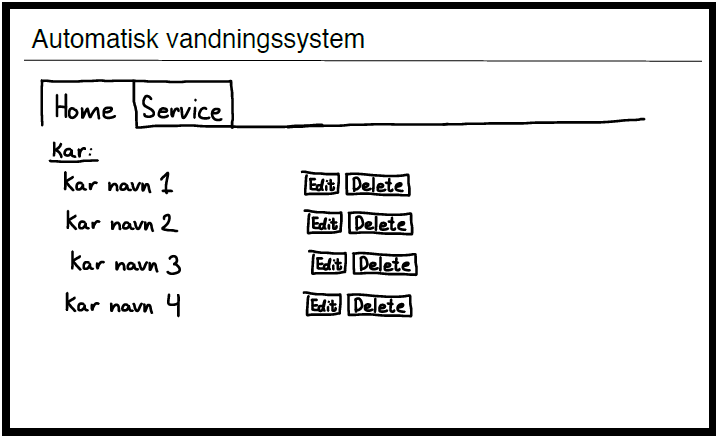
\includegraphics[width=0.7\textwidth]{Kravspecifikation/Interface/photo/index.PNG}
    \caption{AVS Interface - home}
    \label{fig:index}
\end{figure}
På Figur \ref{fig:index} kan brugeren se en liste over de kar der er oprettet, hvor de forskellige kar kan tilgås hvis brugeren klikker på det ønskede kar. 
\\\\
Under service har teknikeren mulighed for at oprette et \gls{kar}, hvor han indtaster adresse, navn og derefter trykker opret \gls{kar}. hvorefter karet kommer frem på listen over \gls{kar}. ydermere er der en delete og edit knap uden for hvert \gls{kar} så teknikeren har mulighed for at slette et \gls{kar} eller redigerer navnet. 
\\\\
Når brugeren trykker på et \gls{kar} tilgår han/hun et interface for \gls{kar}et, som kan ses på Figur \ref{fig:kar}. 
\begin{figure}[H]
    \centering
    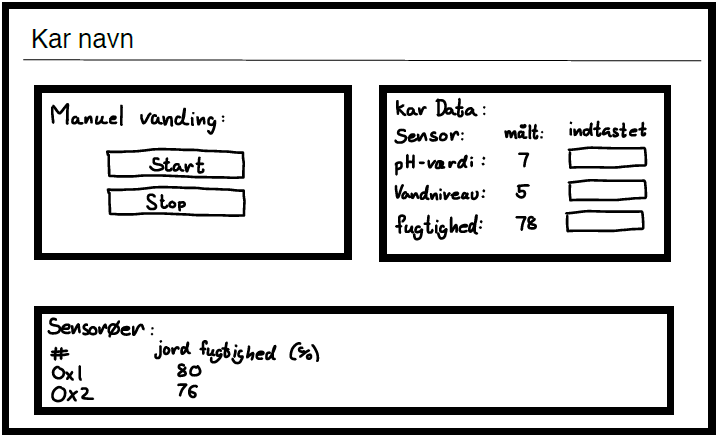
\includegraphics[width=0.7\textwidth]{Kravspecifikation/Interface/photo/kar.PNG}
    \caption{AVS Interface - kar}
    \label{fig:kar}
\end{figure}

I feltet øverste til venstre er der mulighed for manuel vanding, hvor brugeren trykker på start når han/hun vil starte den manuelle vanding. For at stoppe den manuelle vanding trykke på bruger på stop.   
\\\\
I feltet øverst til højre har brugeren mulighed for at indtaste de ønskede data og aflæse de data der kommer fra de forskellige sensor. 
\\\\
I det nederste felt kan der ses en liste over \gls{sensoroe}erne hvor brugeren kan aflæse de data der kommer fra de forskellige sensor.   
